\chapter{Experiment}
\label{ch:exp}
In the experiment an FTB-300 ``Universal Test System''by EXFO was used to characterize optical links and an optical network. To perform the OTDR measurements an in the FTB-300 integrated FTB-7323B was used. In the first experimets a model standard link is examined. The OTDR is connected to a spool of fiber by a patchcord. Another patchcord connects the end of the fiber to another spool of fiber. The end of the fiber is terminated by an open APC connector. 

Figure \ref{fig:1_line} shows the OTDR measurement for the setup. The measurement complete measurement settings can be found in the appendix.
At the distance near $x$~=~0 there is a large reflection caused by the OTDR. The range from $ 0.5$~km$~ < x < 10.5$~km shows the first 10~km spool of fiber. The slope is caused by Rayleigh scattering (cf. {\ref{loss}}). At $x = 10.5~$km a step in the measurement can be observed. At this location the spool of fiber is connected to another spool using a patchcord and APC connectors. This connectors lead to losses. 
The range from $10.5$~km~$ < x < 21$
~km shows the second spool of fiber. At $x = 21$~km the signal drops significantly at the end of the line.


\begin{figure}[h]%
\centering
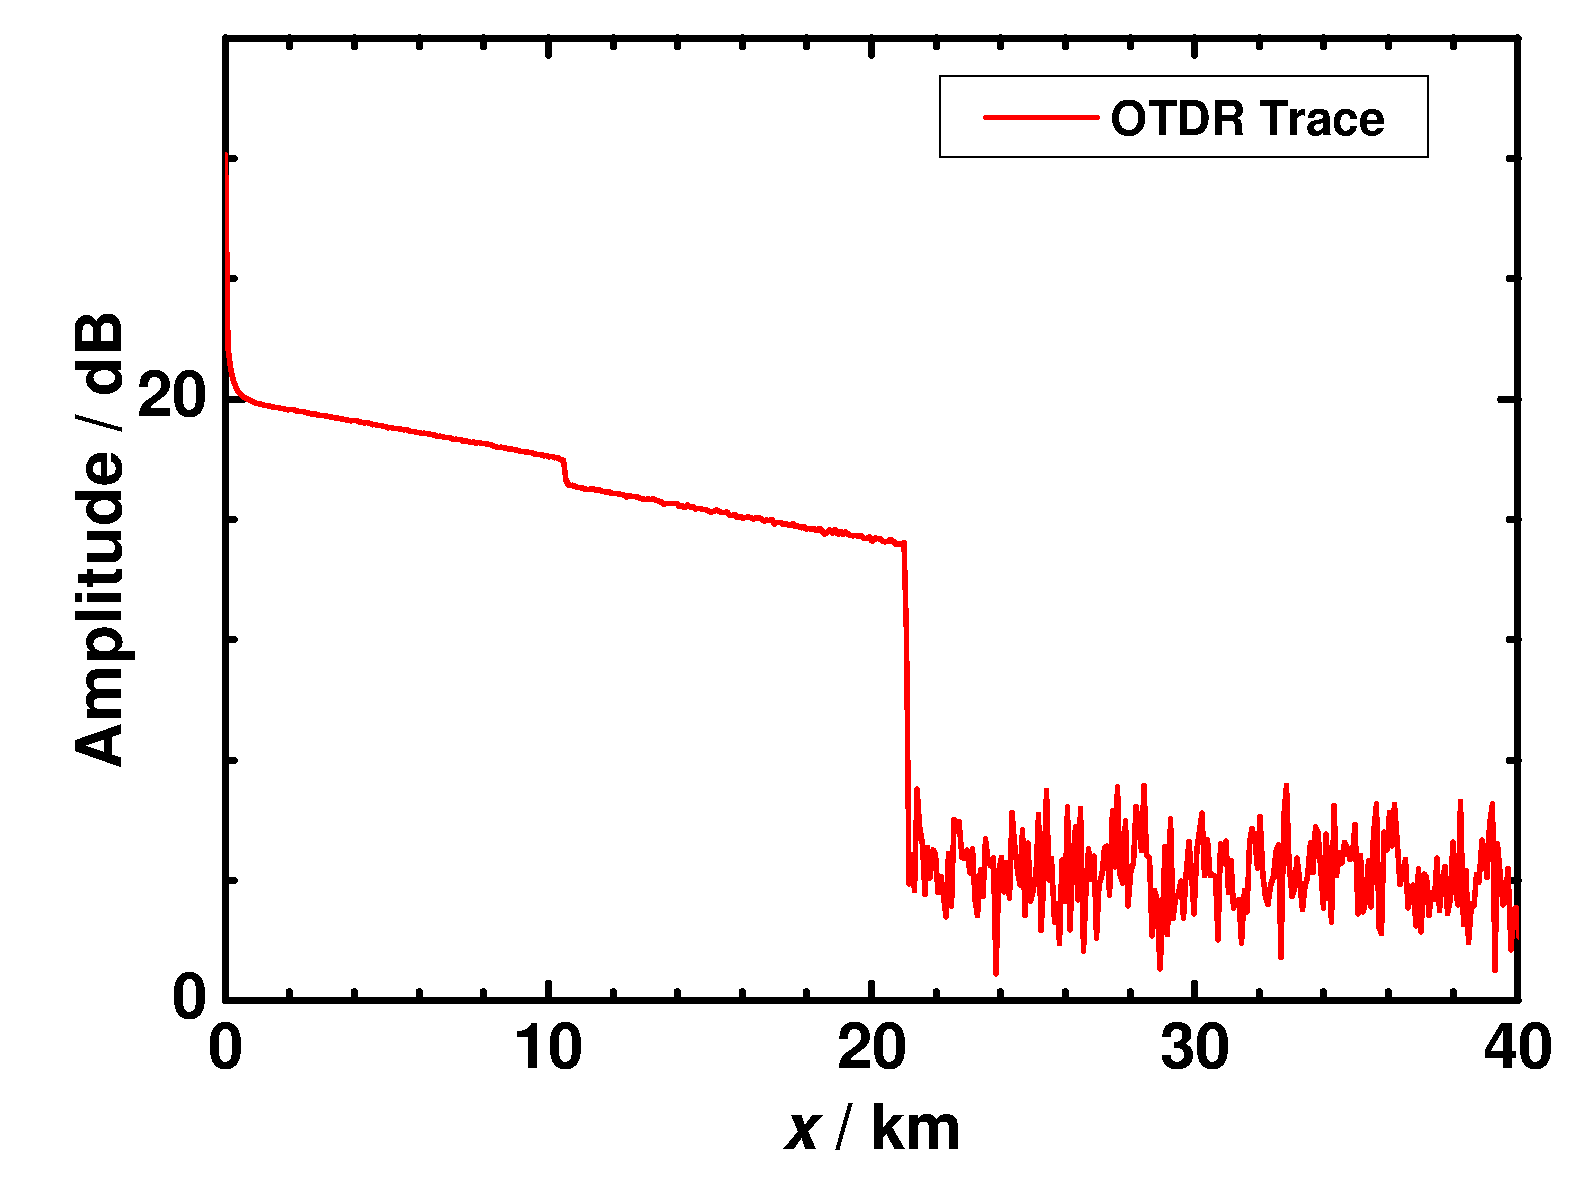
\includegraphics[width=.6\columnwidth]{grafiken/1_line.pdf}%
\caption{Backscattered signal of the setup. (TRACE008)}%
\label{fig:1_line}%
\end{figure}
\newpage

\section{Effects of OTDR measurement parameters on the measurements}
In the first task the effects of the OTDR measurement parameters on the measurement was analyzed. 
The following parameters were set:
\begin{itemize}
	\item \textbf{Wavelength} - The FTB-300 is able to measure with two different wavelength. At the zero dispersion wavelength $\lambda ~=~1310~$nm  of silica based optical fibers and at $\lambda~=~1550$~nm the minimum-loss window for silica based optical fibres.
	\item \textbf{Pulse Width} - The pulse width determines for one thing the resolution of the OTDR (cf. \ref{sec:resolution}), for another thing the maximum measurement distance. 
	\item \textbf{Integration Time} - The OTDR does several measurements and integrates over the preset time to reduce noise. 
\end{itemize}

To determine the effects of the pulse length on the measurement several different length were tested. To demonstrate the effects traces of 5 different pulse length are put into one graph (eg. \ref{fig:1_time}). The integration time for all traces was 30~s. The complete data can be found in the appendix.

Comparing the different traces shown in figure \ref{fig:1_time} leads to the fact, that longer pulses in time lead to an higher signal amplitude. This is obvious since this pulse carries the most energy compared to the other pulses. 
The lowest signal amplitude therefore hast the smallest measured pulse, with a pulse width of $t\i{pulse}$~=~10~ns. But due to the low energy the small pulse carries the signal of short pulses shows higher influence of noise than the longer pulses. 


\begin{figure}[h]%
\centering
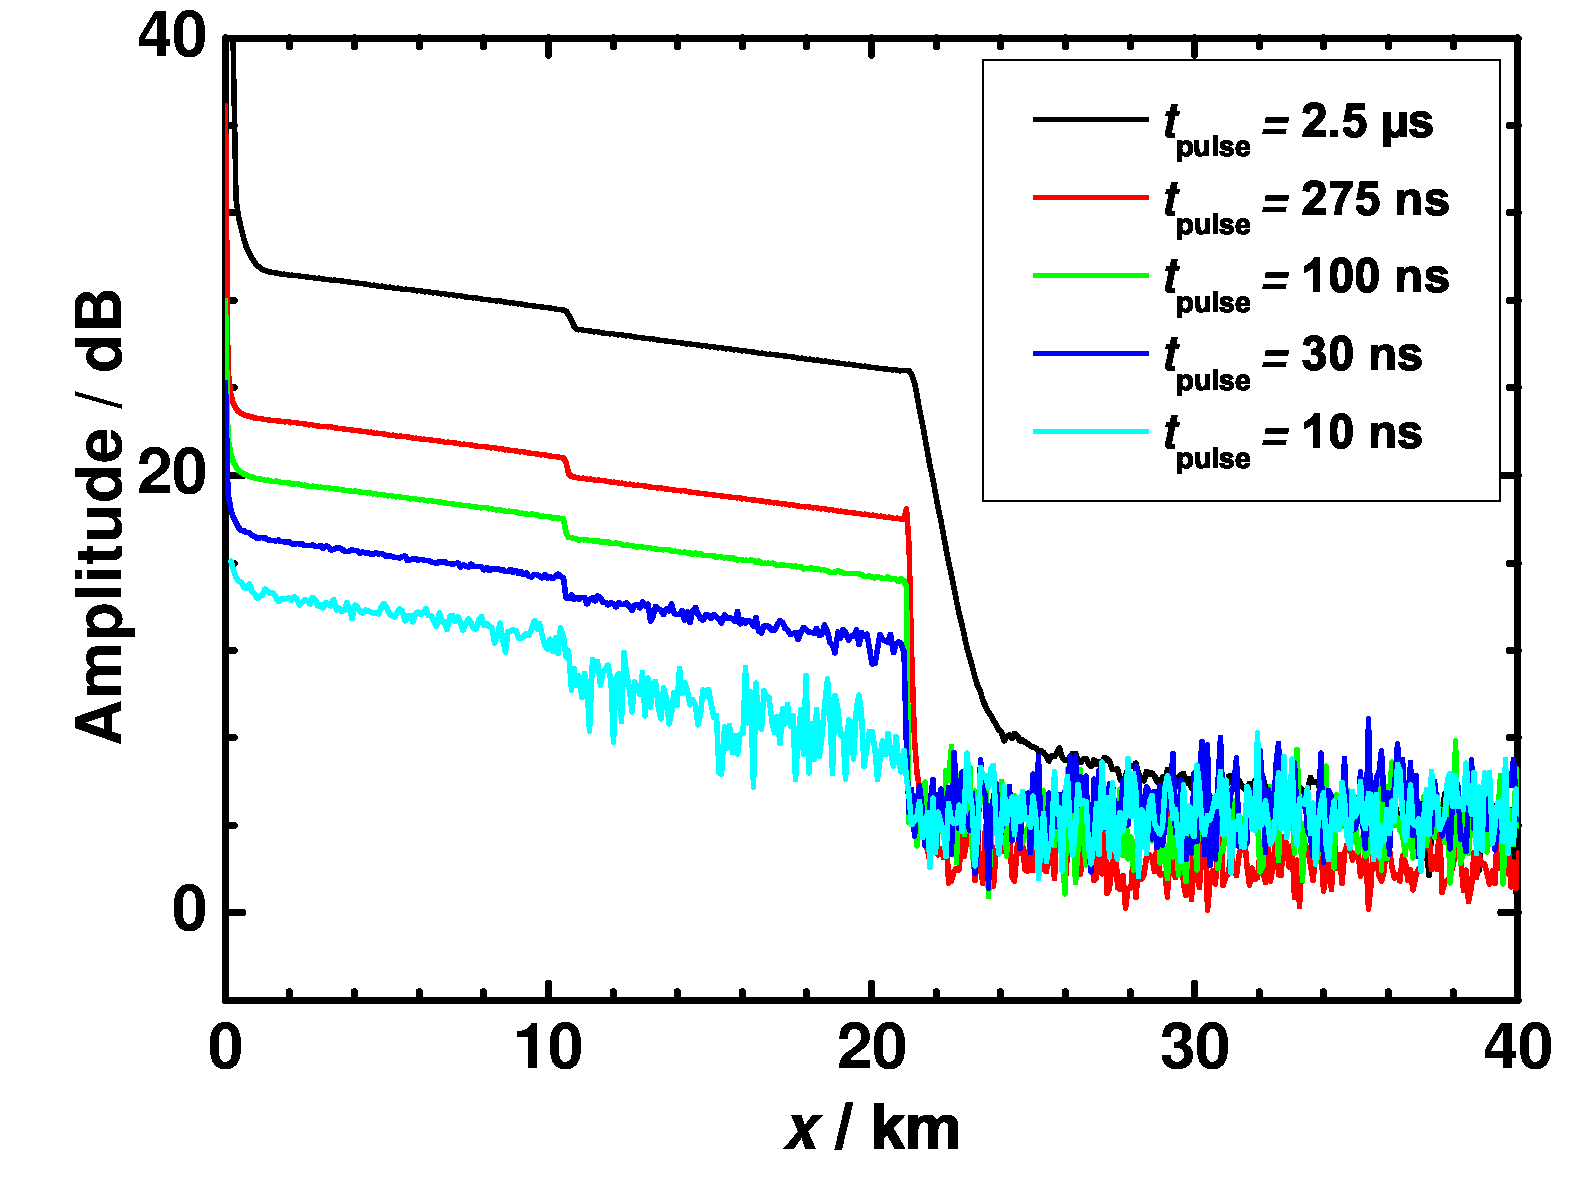
\includegraphics[width=.6\columnwidth]{grafiken/1_time.pdf}%
\caption{Backscattered signal for different pulse widths. (2.5 $\upmu$s: TRACE000, 275 ns: TRACE001, 100~ns: TRACE002, 30~ns: TRACE003, 10~ns: TRACE004). All measurements with an integration time of 30~s.}%
\label{fig:1_time}%
\end{figure}
\newpage

At a distance of $x$~$\approx$~20~km the end of the line can be observed.
The trace of the long pulse shows a large dead zone compared to the other. The signal needs up to 5~km to reach the low signal value the other traces show at this distance. 


To achieve the best performance a compromise between a heigh resolution (small pulse) and a low noise level (large pulse) needs to be found.

To reduce the noise level of the small pulses the integration time can be enlarged.therefore a pulse lenght of 100~ns was selected and the integration time was varied from 30~s to 2~min. 


\begin{figure}[t]%
\centering
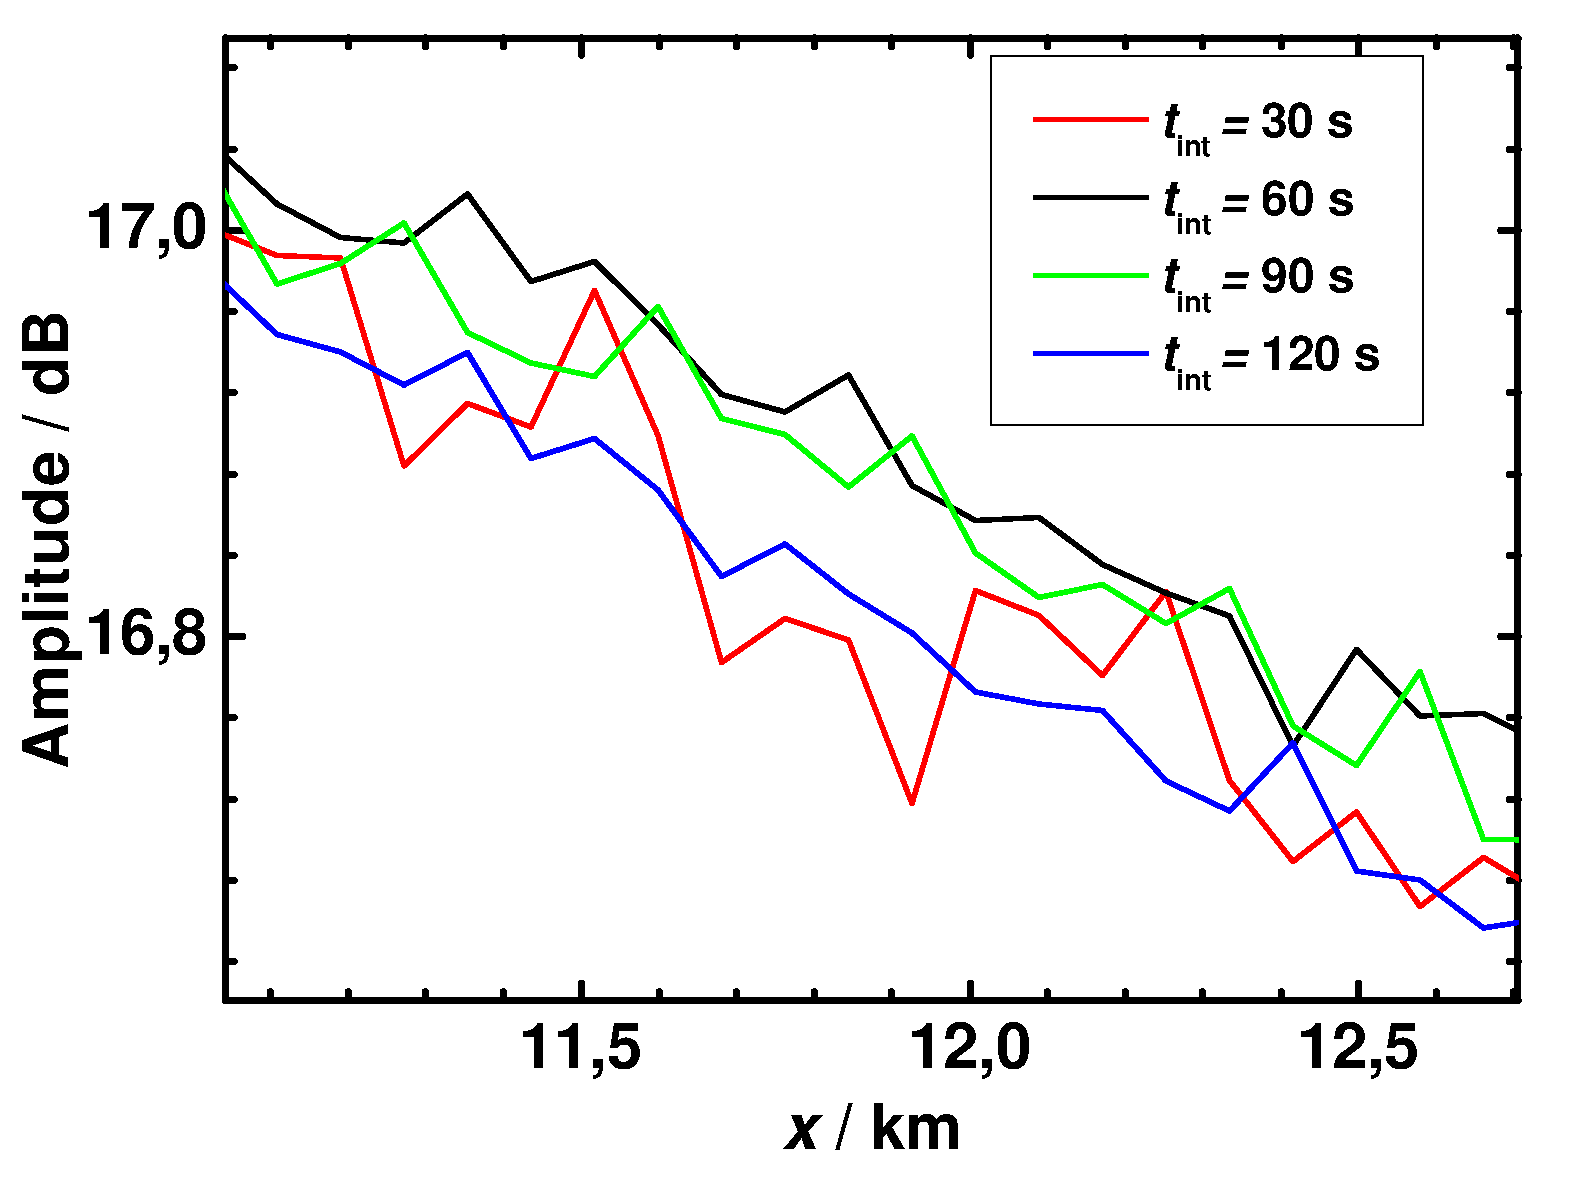
\includegraphics[width=.6\columnwidth]{grafiken/1_integration.pdf}%
\caption{Backscattered signal for different integration times. (30 s: TRACE009, 60 s: TRACE008, 90~s: TRACE010, 120~s: TRACE011). All measurements with a pulse width of 100~ns.}%
\label{fig:integration}%
\end{figure}

Figure \ref{fig:integration} shows a detail of the traces with a 100~ns pulse width for different integration times. The complete data can be found in the appendix.

Changing the integration time leads to a variation of the noise level. An integration time of 30~s leads to an variation of $\sim$0.1~dB. A longer integration time results in a lower variation of the signal. 
Doubling the integration time to 60~s gives an variation of the signal of $\sim$0.02~dB. Increasing the integration time even further gives nearly no improvement of the signal variation but leads to long measurement times.
For this reason the the integration time was set to 1 minute and since the trace with a pulse with 100~ns pulse width shows low noise and a good resolution those parameters were chosen for the following measurements.

Last the influence of the wavelength was examined. Figure \ref{fig:1_lambda} shows the OTDR measurement for the two different wavelenght. Both traces were measured with a pulse width of 100~ns and an integration time of 1 minute. The complete data can be found in the appendix.

\begin{figure}%
\centering
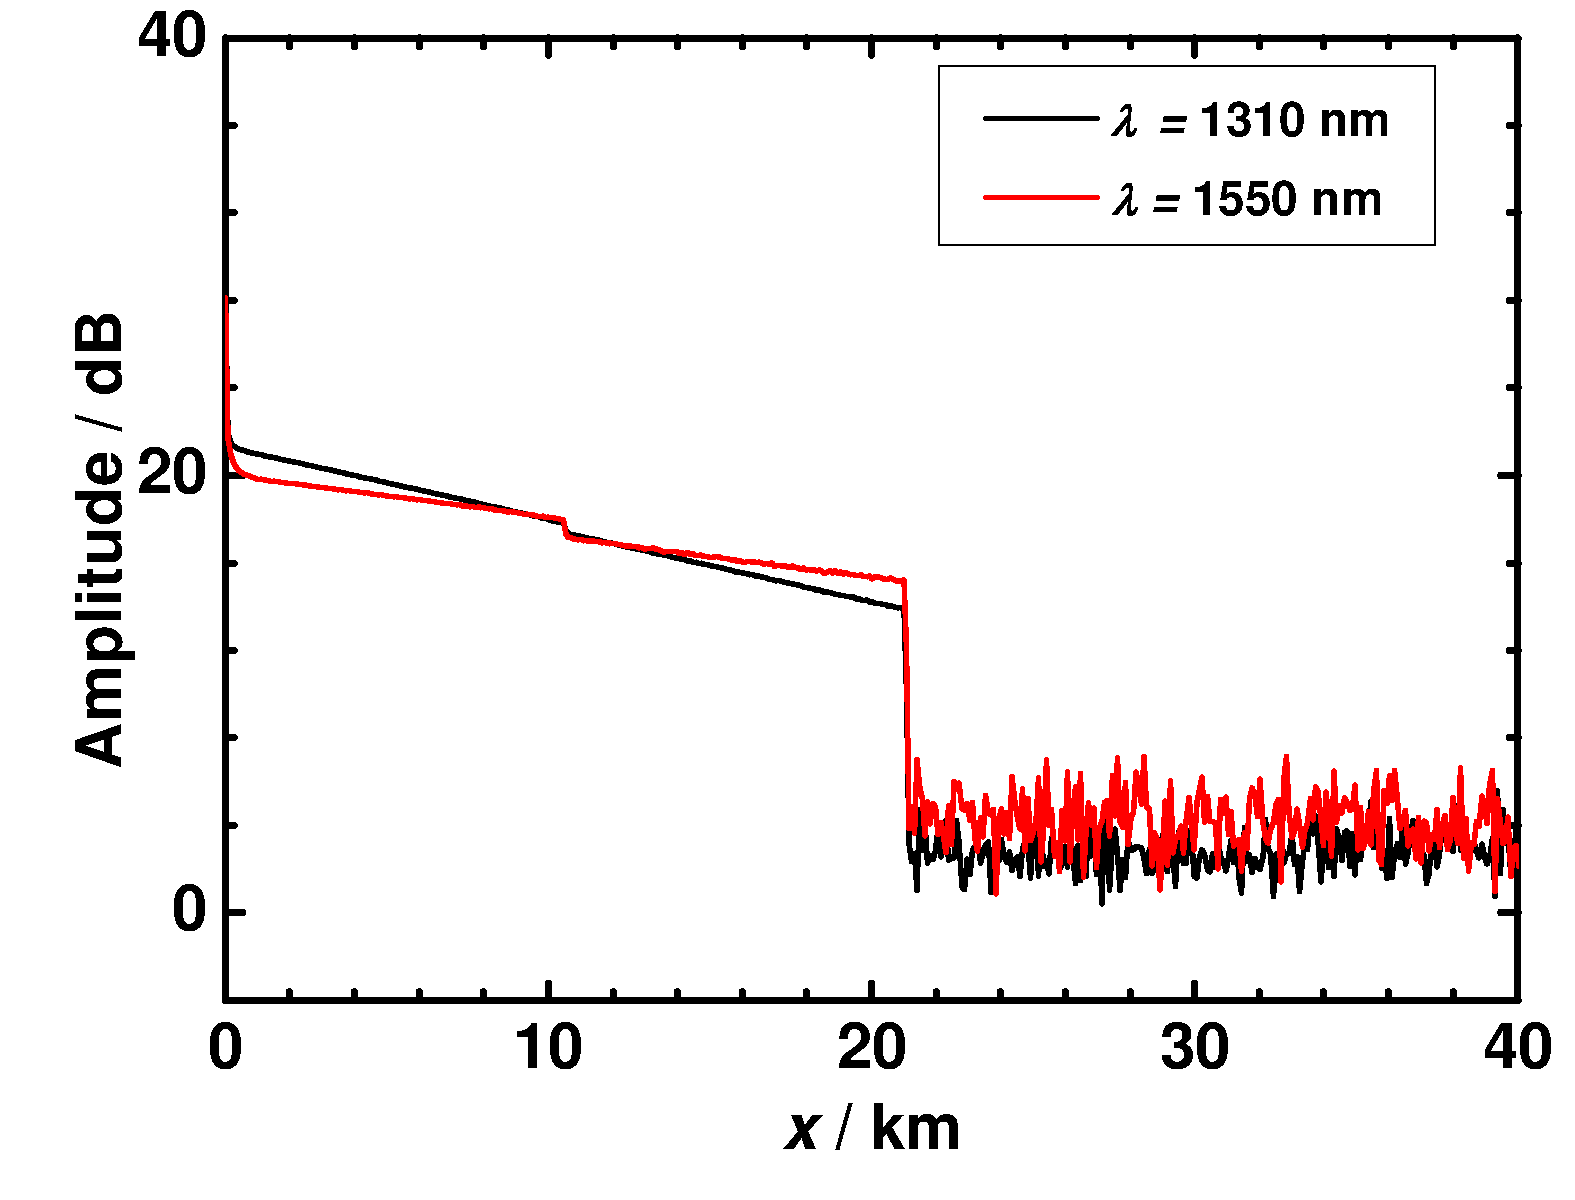
\includegraphics[width=.6\columnwidth]{grafiken/1_lambda.pdf}%
\caption{Backscattered signal for different wavelengths. (1310~nm: TRACE012, 1550~nm: TRACE008). Both measurements with a pulse width of 100~ns and an integration time of 1 minute.}%
\label{fig:1_lambda}%
\end{figure}

Using the EXFO OTDR FTB-7000 software the attenuation of the optical fiber at both wavelengths can be measured at the slopes of the trace. Table \ref{tab:1_daempfung} shows the attenuation at both wavelenghts.

\begin{table}[h]%
\centering
\caption{Attenuation of the optical fiber}
 
\begin{tabular}{cc}

\toprule

$\lambda$	& Attenuation\\
\midrule
1310 nm & 0.34 dB / km\\
1550 nm& 0.19 dB / km\\
\bottomrule 
\end{tabular}
\label{tab:1_daempfung}
\end{table}

The fiber shows a larger attenuation at $\lambda~=~$1310~nm than at $\lambda~=~1550$~nm. This behaviour is expected since the minimum-loss window for silica based optical fibers is at this wavelength. 



\section{Effects of a loose connector on the measurements}
\label{connectors}
\begin{figure}%
\centering
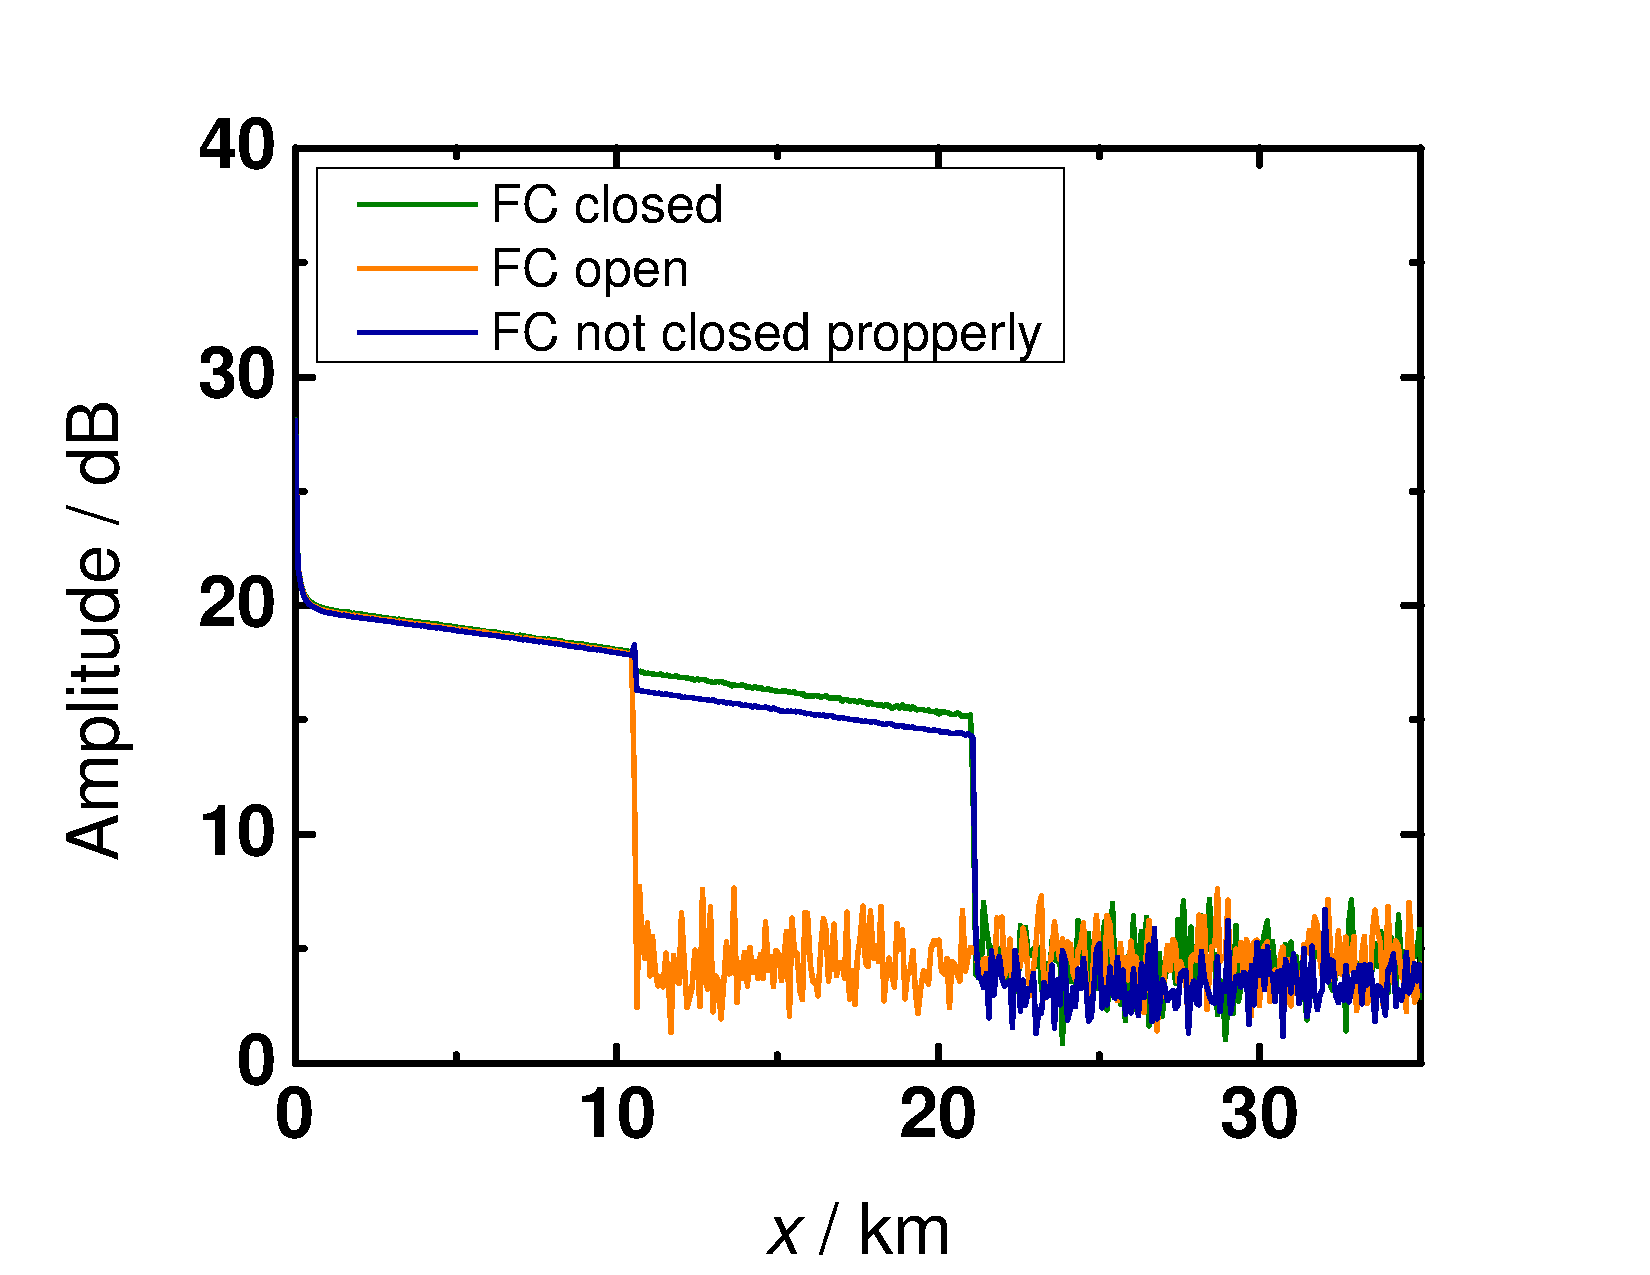
\includegraphics[width=.7\columnwidth]{grafiken/Connector.pdf}%
\caption{}%
\label{fig:connector}%
\end{figure}

In this experiment a connector at the patchcord between the two fibers is loosend. The measurements for this are shown in figure \ref{fig:connector}. The blue curve shows the signal of the link with a closed fiber. When the connector is loosend the losses of the connection increases (green curve). When the connector is loosend further the losses of the connection become so big, that they can't be measured with the OTDR system (orange curve). 

The losses at the connection of a not propperly closed fiber are caused primarily by the end gap between the fibers. Since the light emitted by the end of a fiber spreads conicaly, a higher amount of light misses the core and is not coupled in the other fiber\footnote[4]{http://www.lanshack.com/fiber-optic-tutorial-termination.aspx}.

Using the 4 point measurement of the OTDR the Losses for the closed connector are measured as 0.8~dB. For a not propperly closed connection a loss of 2.6~dB is measured. For a connector loosend further the losses at the connection are greater than 9~dB, so that the backscattering at the end of the fiber couldn't be detected.

\section{Effects of a bend on the measurements}
To calculate the effects of bends in the optical fiber the patchcord between the two 10~km spools of optical fiber was bent. To produce repeatable measurements supplied loops with 15~mm, 20~mm, 30~mm and 40~mm diameter were used. The fiber was wound 1, 2 and 3 times around each loop. 

The first measurements were performed with a pulse width of 100~ns. Bends with higher losses this pulses carried not enough energy. At this measurements the signal after the bend is to low to get a clear signal. For this reason the pulse length was adjusted to 275~ns. 
But even that pulse was to short for high-lossy bends. So the pulse width was enlarged even further to 1~$\upmu$s. 
Since the pulse width does not affect the losses in the fiber measurements performed with different pulse widths can be compared regarding the losses in a bend waveguide.

\begin{table}%
\centering
\caption{Losses based on bends in the waveguide.}
 
\begin{tabular}{cccc}

\toprule

bend radius	& number of turns	&	loss &measurement\\
\midrule
15~mm	&	1	& 6.9~dB	&TRACE032\\
15~mm	&	2	& 12.2 dB	&TRACE031\\
15~mm	&	3	& >14~dB	&TRACE033	\\
\midrule
20~mm	&	1	& 2.6~dB	&TRACE026	\\
20~mm	&	2	&3.7~dB	&TRACE027\\
20~mm	&	3	& 8.2~dB&TRACE029	\\\midrule
30~mm	&	1	&0.9~dB	&TRACE030	\\
30~mm	&	2	& 1.0~dB&TRACE034	\\
30~mm	&	3	& 1.1~dB&TRACE035	\\\midrule
40~mm	&	1	&	0.9~dB&TRACE036	\\
40~mm	&	2	&0.9~dB	&TRACE037	\\
40~mm	&	3	& 0.9~dB&TRACE038	\\
\bottomrule 
\end{tabular}
\label{tab:3_daempfung}
\end{table}
% Table \ref{tab:3_daempfung} compares the losses based on bends in the waveguide. The measured data can be found in the appendix. As expected (cf. \ref{bend_loss}) the smallest bend diameter of $d=15$~mm leads to the highest losses. Every turn of the fiber increases the losses. The losses when the fiber is turned three times around the loop with $d=15$~mm are to high to measure with a pulse length of 1~$\upmu$m.

Table \ref{tab:3_daempfung} compares the losses based on bends in the waveguide. The measured data can be found in the appendix. As expected (cf. \ref{bend_loss}) the smallest bend diameter of $d=15$~mm leads to the highest losses. With a larger bend diameter the losses are getting lower. A higher number of turns causes a longer way trough the bends and thus increases the losses. At a diameter of $d=15$~mm the losses are to high to be measured with a pulse length of 1~$\upmu$m. 

Figure \ref{fig:3_bend} illustrates the dependence of the losses on the bend diameters and the number of turns $n$. The diameter of $d = 30$~mm shows only a small increase of attenuation per turn. A bend diameter of 40~mm finally leads to a loss of 0.9~dB. This can be compared to the losses of the connectors (cf. \ref{connectors}) with 0.8~dB. Since the number of turns have no influence on the losses in this case one can say that a bend of a diameter of 40~mm or larger causes no additional loss.



\begin{figure}%
\centering
%\begin{adjustwidth}{0cm}{0cm}
	\subfloat[]{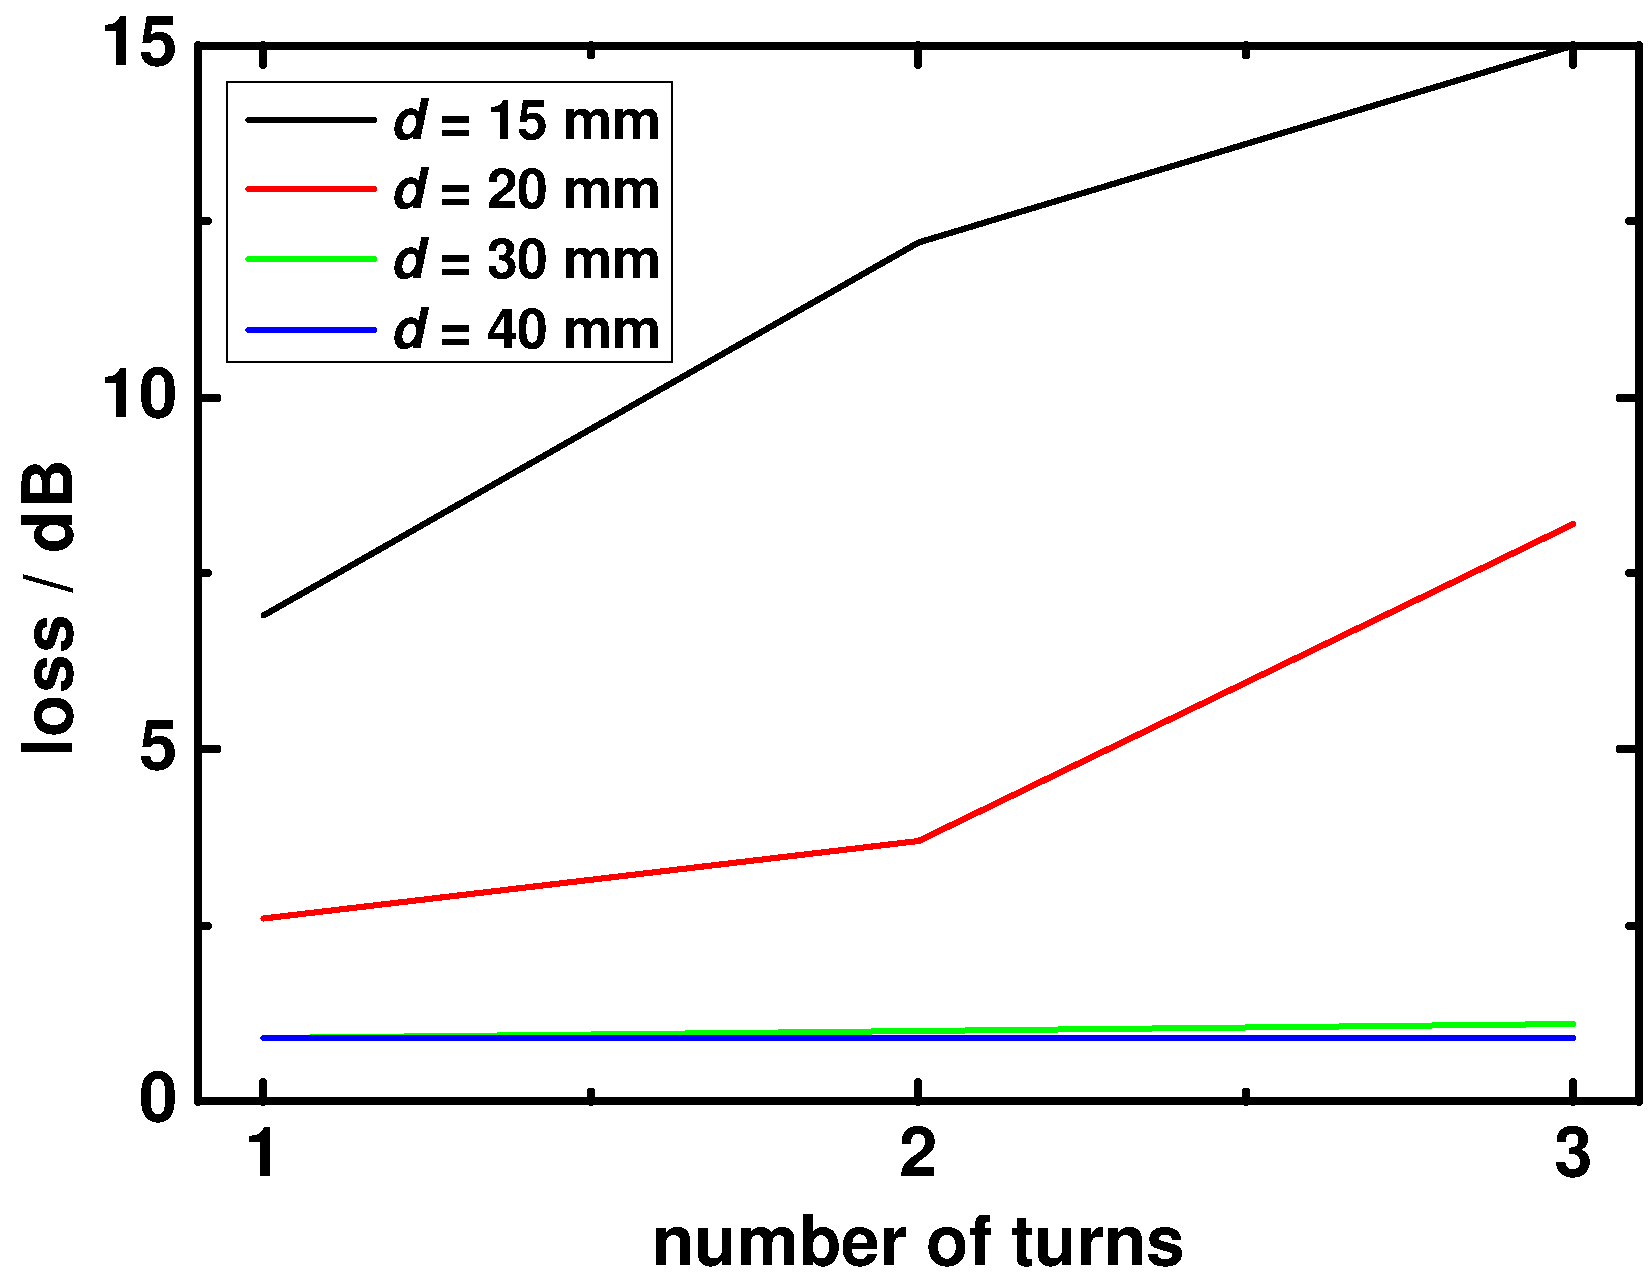
\includegraphics[totalheight=5 cm]{grafiken/3_radii.pdf}\label{fig:3_radii}}\qquad
	\subfloat[]{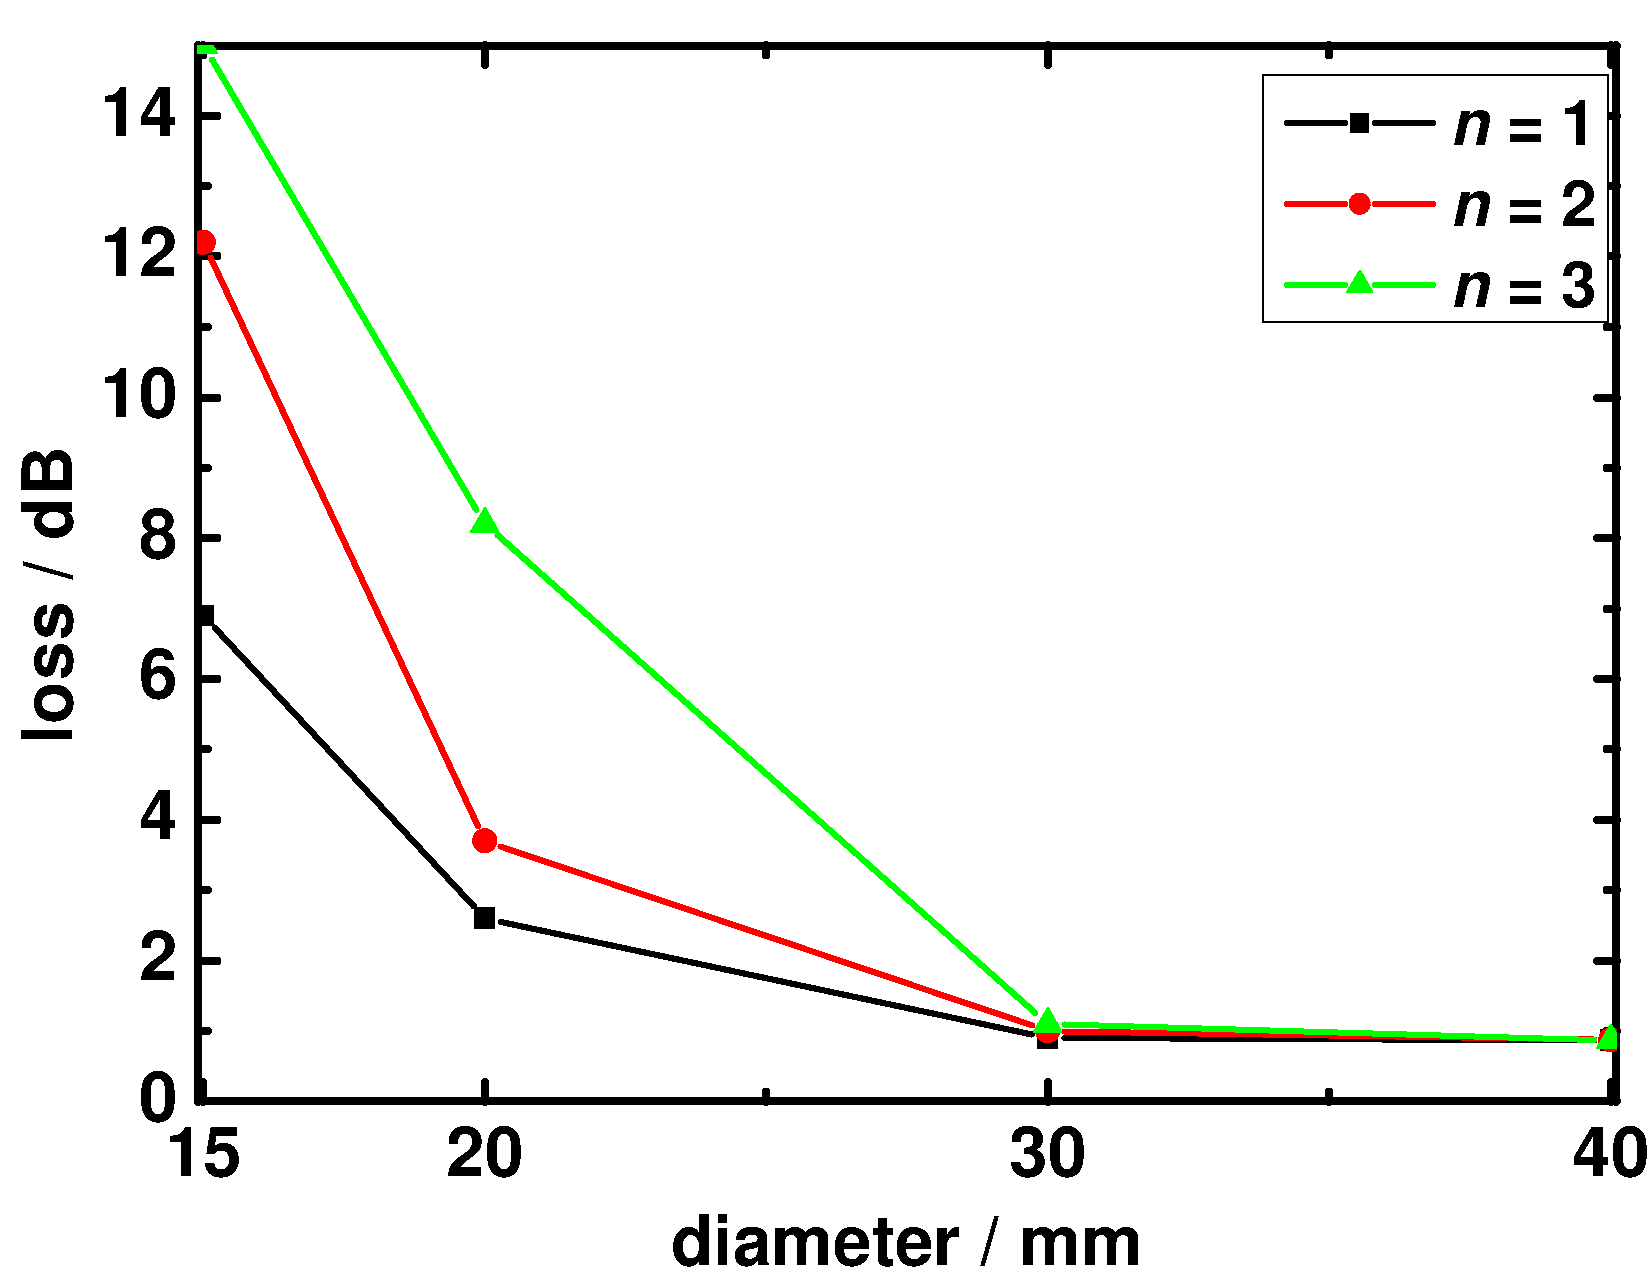
\includegraphics[totalheight=5 cm]{grafiken/3_diameter.pdf} \label{fig:3_diameter}}\\
\caption{Losses in a bend waveguide with different diameters and number of turns. \textbf{(a)} loss vs. number of turns $n$,  \textbf{(b)} loss vs. bend diameter.}%
\label{fig:3_bend}%
\end{figure}



%\begin{figure}%
%\centering
%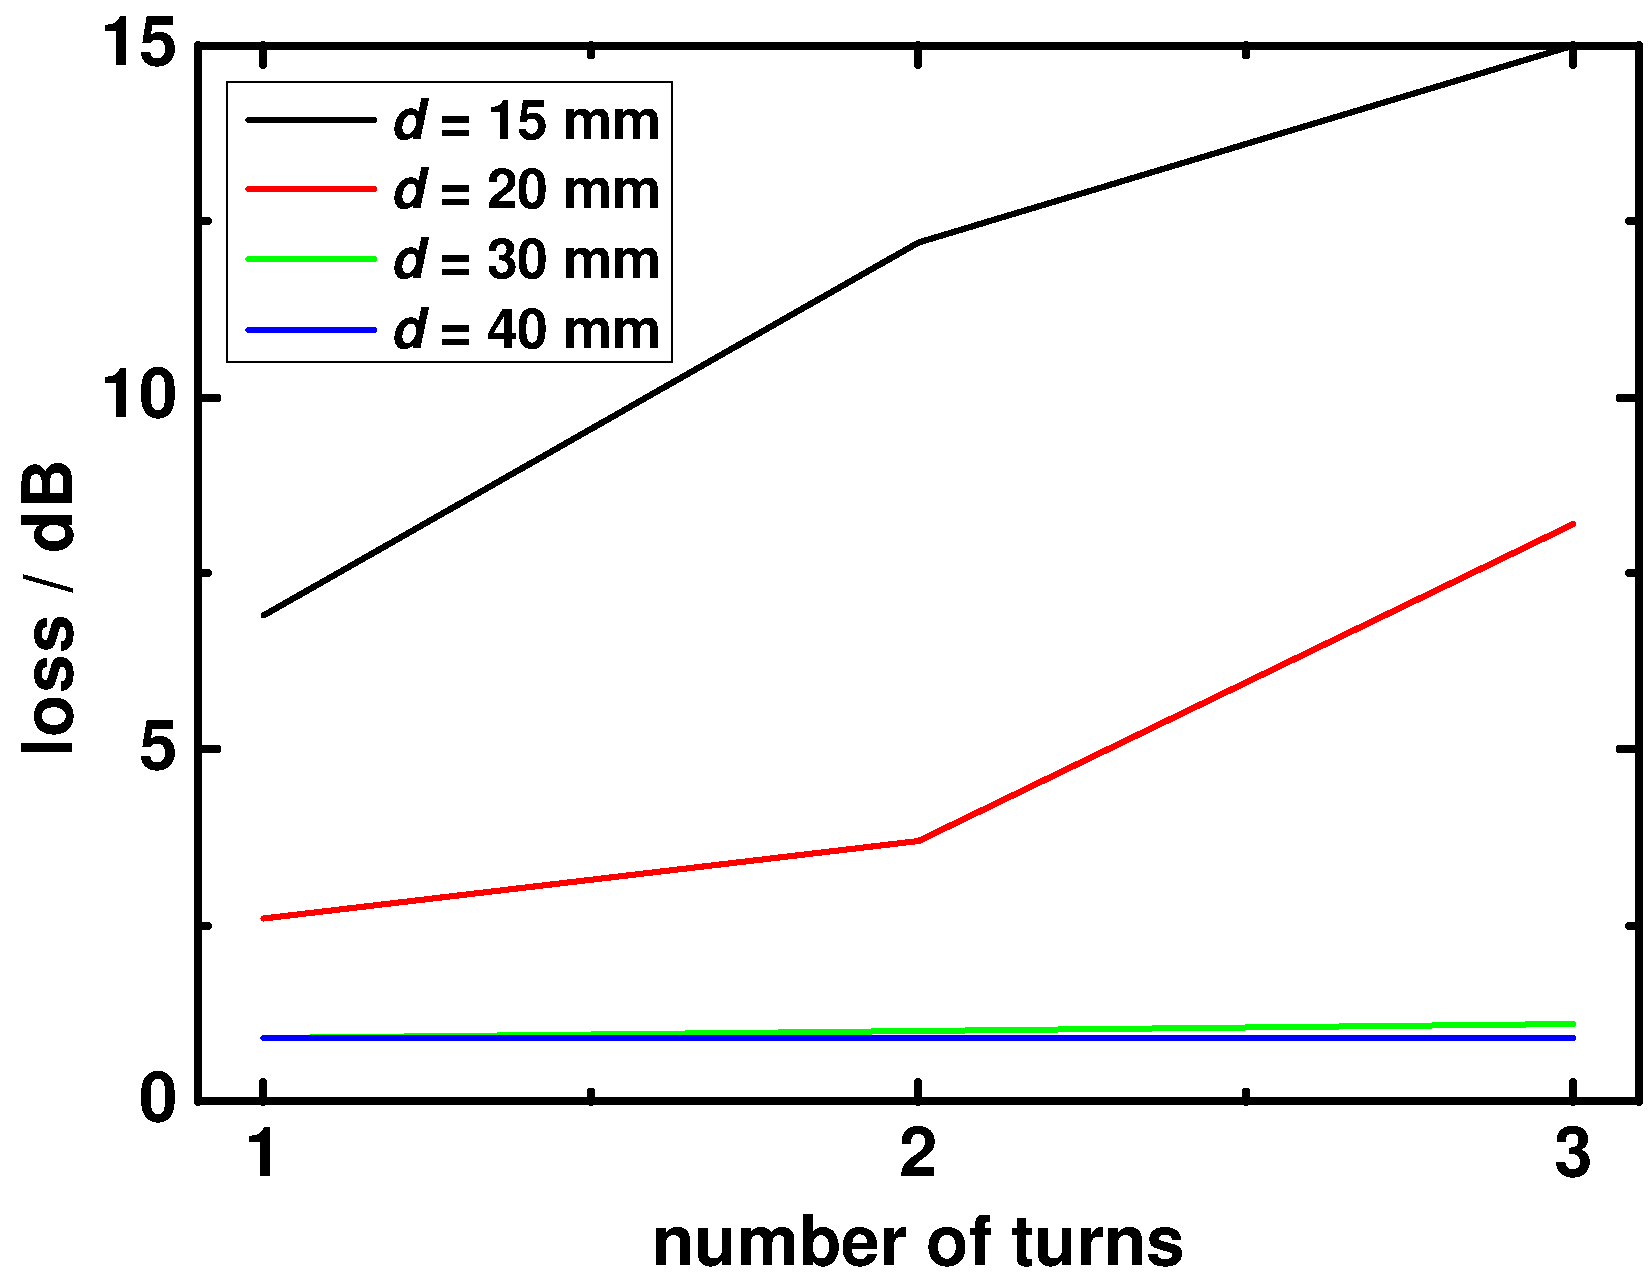
\includegraphics[width=.6\columnwidth]{grafiken/3_radii.pdf}%
%\caption{Losses in a bend waveguide with different diameters and number of turns.}%
%\label{fig:3_radii}%
%\end{figure}

% With a larger bend diameter the losses are getting lower. A bend diameter of 40~mm leads to a loss of 0.9~dB. This can be compared to the losses of the connectors (cf. \ref{connectors}) with 0.8~dB. Since the number of turns have no influence in the losses one can say that a bend of a diameter of 40~nm or larger causes no additional loss.
% 
% 
% 
% Figure \ref{fig:3_bend} illustrates the dependence of the losses on the bend diameters and the number of turns $n$. As noticed before a smaller bend diameter leads to higher losses based on the bends. A higher number of turns causes a longer way trough the lossy section. The diameter of $d = 30$~mm shows only a small increase of attenuation per turn. Probably a little bit larger diameter leads to no additional losses per turn.

% \todo{take a resume with an overview data plot!!!}



\section{Effects of an open end with a PC connector}
In the next task of the experiment the APC connector at the end was changed with a PC connector. The difference between the PC and APC is the angle at the end (0� for PC and 8� APC) The simulation was run again with pulse width 1.0 $\upmu$s and wavelength 1550 nm. The results are seen in figure \ref{fig:4_reflection}.


\begin{figure}%
\centering
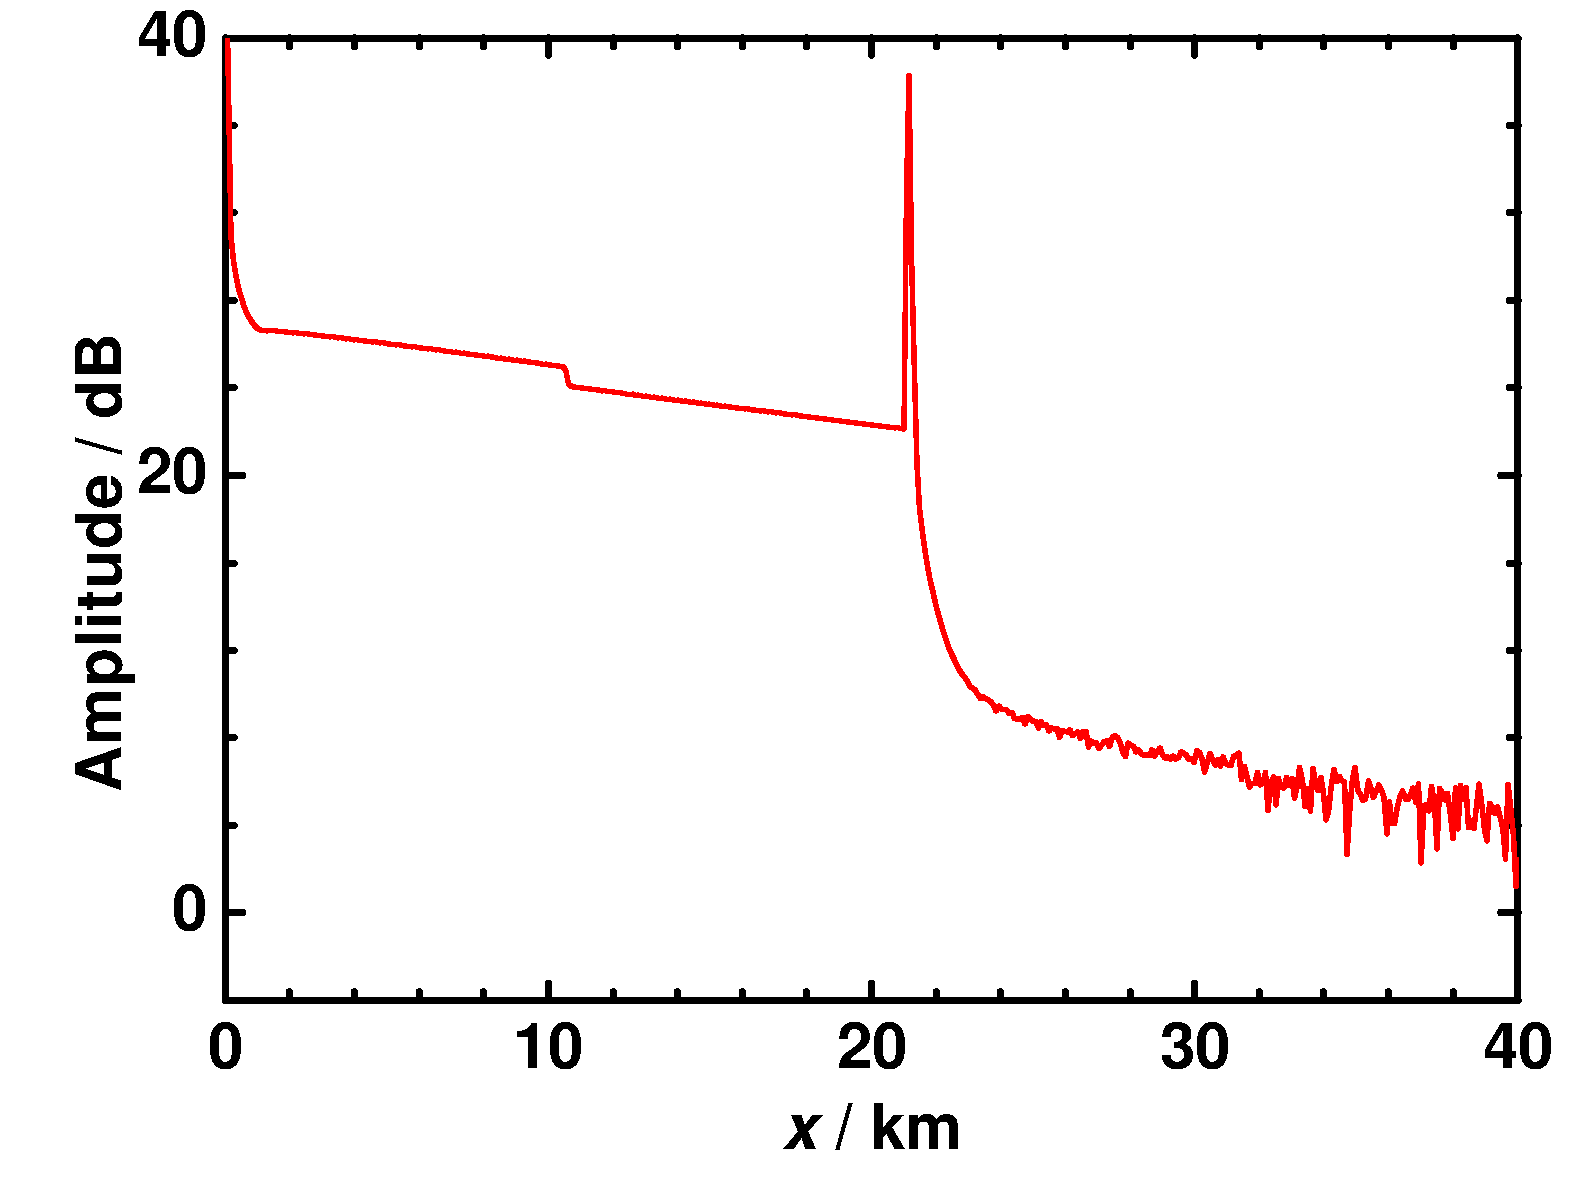
\includegraphics[width=.6\columnwidth]{grafiken/4_reflection.pdf}%
\caption{OTDR signal with an PC connector at the end. (TRACE039)}%
\label{fig:4_reflection}%
\end{figure}

At 21st km where APC connector was replaced with a PC a high reflection peek can be seen. It is due to the fact that the PC connector has a 0� angle. This simplifies the Fresnel equation to the following:

\begin{equation}
R = \left(\frac{n_1-n_2}{n_1+n_2}\right)^2
\label{eq:}
\end{equation}
For refractive indexes n1 and n2 are respectively 1 and 1.43 (air, fused silica) which leads to R=3~\% which is quite inaccurate compared to the result from the OTDR -16~\%.
\todo{Why? The sistem is not ideal?}
\comwo{Sebastian: Du als alter Fiber-Experte musst das doch wissen?}

\section{Analysis of an optical network}
For the last part three different measurements at different pulse widths were performed before the right resolution was chosen.  The results for pulse width of 275ns where chosen as they give the most distinguishable drops and peaks at the highest possible resolution. 

\begin{figure}%
\centering
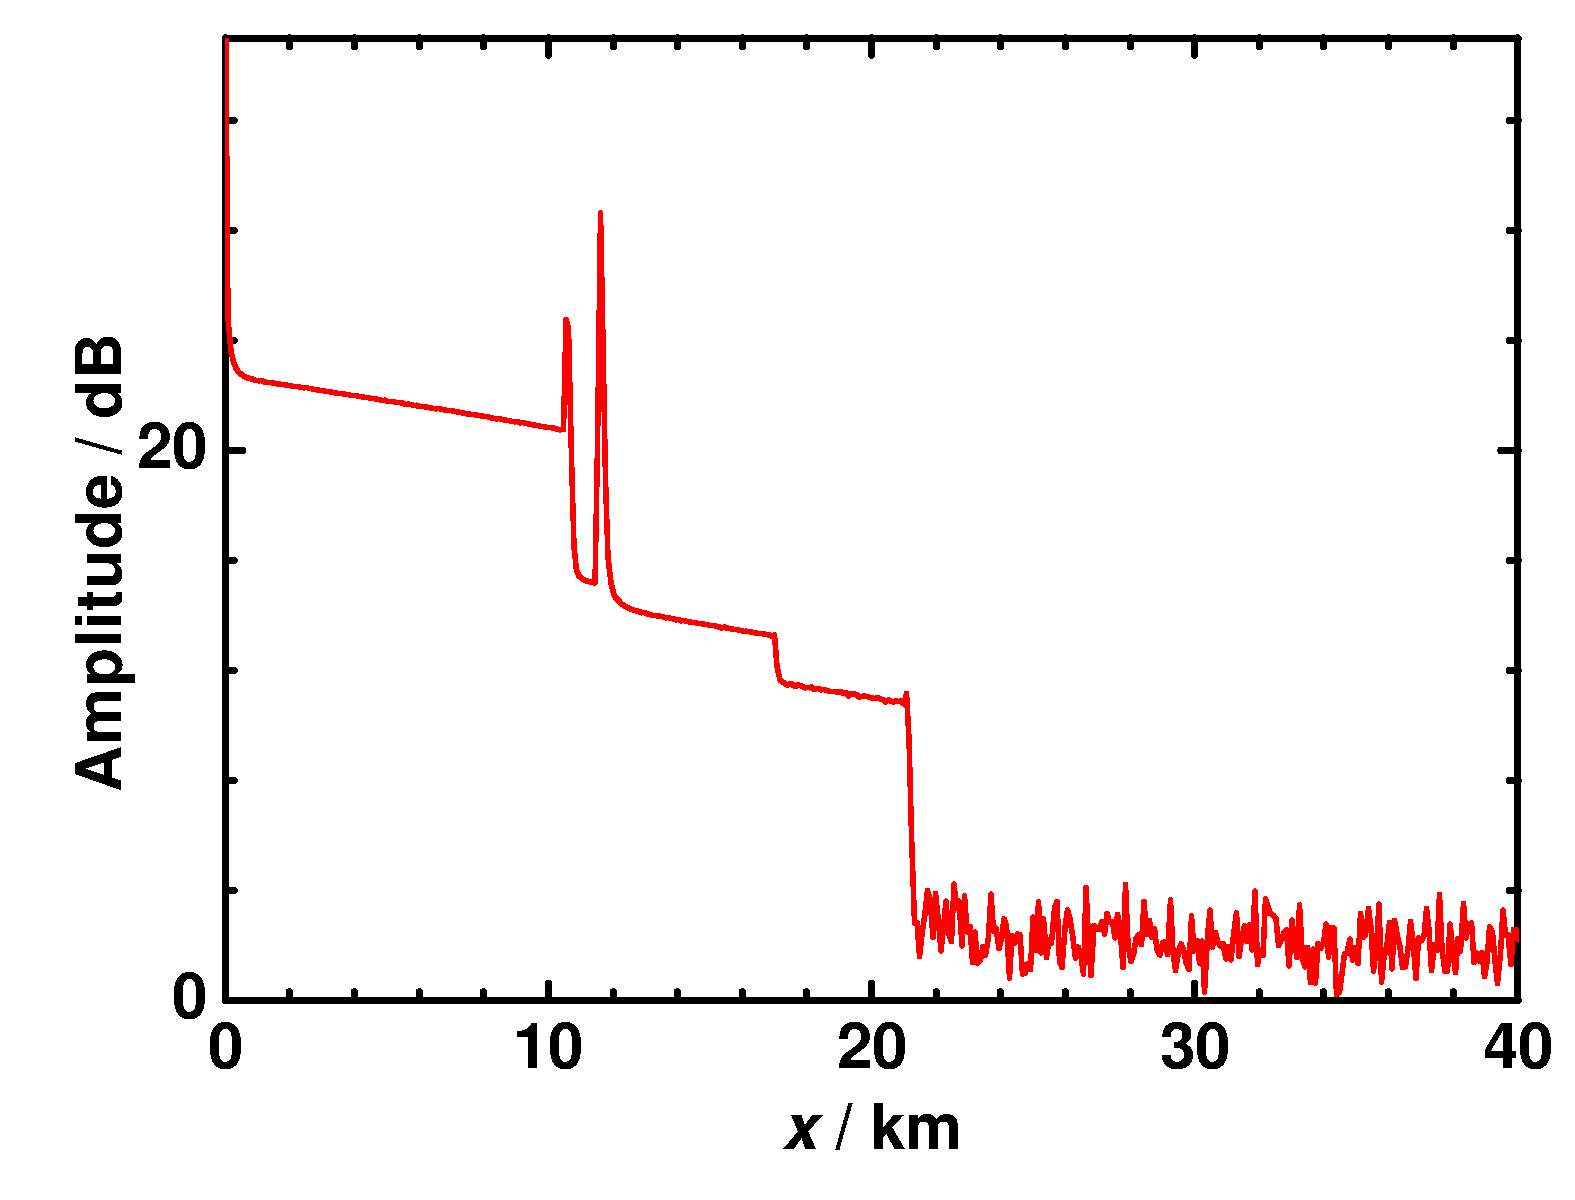
\includegraphics[width=.6\columnwidth]{grafiken/5_line.pdf}%
\caption{OTDR signal of a test network. (TRACE42)}%
\label{fig:5_line}%
\end{figure}

Figure \ref{fig:5_line} shows the measured data. After 10~km of fiber a peak with a sudden drop of power right afterwards can be seen. This leads to the assumption that there is a PC connector and splitter. The drop is about 9~dB wichs is approximately the attenuation caused by a 1:4 splitter (ideal 1:4 splitter has 6~dB loss).

The large peak at about 12 km leads to the idea that there is a open PC connector. \comwo{Ich denke der connector ist offen, da der peak doch deutlich hoch ist... und wenn wir schon einen splitter dran haben sollten wir auch verschiedene lines sein} 

The small drop at the 17$^{\mathrm{th}}$~km can have several different explanations
\begin{itemize}
	\item A bad connector
	\item An error in the fiber (for example a large bend)
	\item An open APC connector \comwo{Diesen Punkt habe ich eingef�gt, da wir irgendwie sowas mit moritz besprochen hatten, vgl. das untere bild auf dem gescannten zettel} 
\end{itemize}

The end of the whole transmission setup is at 21.1~km which can be easily seen in the picture.

The network topology could be the following:\\
A 10~km spool of fiber followed by a 1:4 splitter. The splitter could be connected to the spool via a PC connector or is reflecting itself. 
At one port of the splitter is a approximately 800~m long fiber with an open PC at the end. 
One port could have a $\sim$9~km long line with an error or a bad connection at the middle of that line. In this case nothing is connected to the two remaining ports of the splitter.
The other case is, that there is one $\sim$9~km long line with no measurable error within the line and an additional line at a third port of the splitter. This third line would than have a length of $\sim$5~km and is ended with an APC connector.

\begin{figure}%
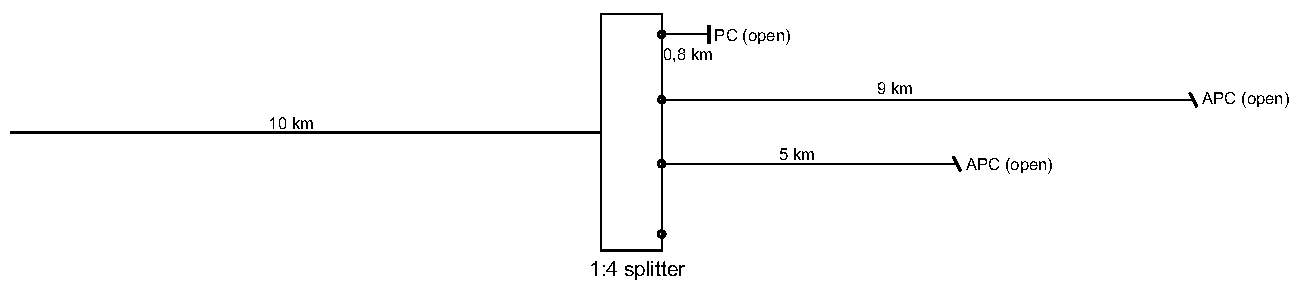
\includegraphics[width=\columnwidth]{grafiken/network.pdf}%
\caption{Possible network topology.}%
\label{fig_5_network}%
\end{figure}

\todo{Appendix nicht vergessen! Am besten die Traces extra auf dem SW drucker ausdrucken und anheften?}
